\documentclass[../../../../main.tex]{subfiles}

\begin{document}

\section*{第1問}

\begin{proof}[解]
$0 \leqq x \leqq 1$, $0 \leqq y \leqq 1$, $2 \leqq z \leqq 3$ \hfill $\dots$ \textcircled{1}

\begin{enumerate}
    \item[(1)] $w = 3 \iff 3(z-y) = z-x \iff 2z = 3y-x$ だが, \textcircled{1}から $4 \leqq 2z \leqq 6$, $-1 \leqq 3y-x \leqq 3$ となるので, $w=3$ となることはない.

    \item[(2)] $\operatorname{Max} w = \dfrac{z}{z-1}$

    \item[(3)] (2)で $z$ をうごかして, $w = 1 + \dfrac{1}{z-1}$ だから, $z=2$ で $\operatorname{max} 2$.

    \item[(4)] $z$ が一定の時 $\dfrac{z-1}{z} \leqq w \leqq \dfrac{z}{z-1}$ だから, $w$ の存在範囲は右図斜線部（境界含む）だから, もとめる $\max k$ は $k = \dfrac{3}{2}$ である.
\end{enumerate}

\begin{center}
\begin{tikzpicture}[scale=1.5, >=stealth]
    % Axes
    \draw[->] (-0.3,0) -- (3.8,0) node[below] {$z$};
    \draw[->] (0,-0.3) -- (0,2.4) node[left] {$w$};
    \node[below left] at (0,0) {$0$};

    % Shaded region domain z in [2, 3]
    \fill[pattern=north east lines, pattern color=gray!60] 
        plot[domain=2:3, smooth] (\x, {\x/(\x-1)}) -- 
        (3, 2/3) -- 
        plot[domain=3:2, smooth] (\x, {(\x-1)/\x}) -- 
        cycle;

    \draw[thick, domain=1.5:3.5, samples=100] plot (\x, {\x/(\x-1)}) node[right] {$w = \frac{z}{z-1}$};
    \draw[thick, domain=1.5:3.5, samples=100] plot (\x, {(\x-1)/\x}) node[right] {$w = \frac{z-1}{z}$};

    % Vertical boundary lines
    \draw[dashed] (2,0) node[below] {$2$} -- (2,2);
    \draw[dashed] (3,0) node[below] {$3$} -- (3,1.5);

    % Ticks on w-axis
    \draw[dashed] (0,2) node[left] {$2$} -- (2,2);
    \draw[dashed] (0,1.5) node[left] {$\frac{3}{2}$} -- (3,1.5);
    \draw[dashed] (0,1) node[left] {$1$} -- (3.5,1);
    \draw[dashed] (0,2/3) node[left] {$\frac{2}{3}$} -- (3,2/3);
    \draw[dashed] (0,0.5) node[left] {$\frac{1}{2}$} -- (2,0.5);
\end{tikzpicture}
\end{center}
\end{proof}

\section*{第2問}

\begin{proof}[解]
\begin{enumerate}
    \item[(1)] まず, $\dfrac{a+b}{2} \geqq \sqrt{ab} \quad \dots$ \textcircled{1} を示す. 両辺正から,
    \[
    \text{\textcircled{1}} \iff (a+b)^2 \geqq 4ab \iff (a-b)^2 \geqq 0
    \]
    だから, \textcircled{1}は成立し, 等号成立は $a=b$ の時.

    さて, $(a,b) = (a+b, c+d)$ として代入すると
    \[
    \dfrac{a+b+c+d}{2} \geqq \sqrt{(a+b)(c+d)} \geqq \sqrt{2\sqrt{abcd} + 2\sqrt{abcd}} \quad (\because \text{\textcircled{1}})
    \]
    \[
    = 2 \sqrt[4]{abcd} \quad \therefore \dfrac{a+b+c+d}{4} \geqq \sqrt[4]{abcd} \qquad \dots \text{\textcircled{2}}
    \]

    \textcircled{2}で $d = \dfrac{a+b+c}{3}$ として代入
    \[
    \dfrac{a+b+c+\frac{a+b+c}{3}}{4} \geqq \sqrt[4]{abc \cdot \frac{a+b+c}{3}} \quad \therefore \dfrac{a+b+c}{3} \geqq \sqrt[4]{abc \cdot \frac{a+b+c}{3}}
    \]
    両辺正から4乗して整理
    \[
    \left(\dfrac{a+b+c}{3}\right)^3 \geqq abc \quad \therefore \dfrac{a+b+c}{3} \geqq \sqrt[3]{abc} \qquad \dots \text{\textcircled{3}}
    \]

    \item[(2)] 
    \[
    P = \dfrac{3a+3b+3c+3d}{12} \geqq \dfrac{\sqrt{ab} + \sqrt{ac} + \sqrt{ad} + \sqrt{bc} + \sqrt{bd} + \sqrt{cd}}{6} \quad (\because \text{\textcircled{1}}) = R
    \]
    \[
    R = \dfrac{2\sqrt{ab} + 2\sqrt{bc} + 2\sqrt{ac} + 2\sqrt{ad} + 2\sqrt{bd} + 2\sqrt{cd}}{12}
    \]
    \[
    \geqq \dfrac{\sqrt[3]{abc} + \sqrt[3]{abd} + \sqrt[3]{acd} + \sqrt[3]{bcd}}{3} \quad (\because \text{\textcircled{3}}) = S
    \]
    \[
    S \geqq \sqrt[4]{abcd} \quad (\because \text{\textcircled{2}}) = Q
    \]
    より
    \[
    P \geqq R \geqq S \geqq Q
    \]
\end{enumerate}
\end{proof}

\section*{第3問}

\begin{proof}[解]
内接円の中心 $O$ から $AB, BC, CA$ に下ろした垂足を順に $H_1, H_2, H_3$ とする. $AC, BC$ に接する円を, 内接円から順に $C_0, C_1, C_2, \dots$ とおく. $C_n$ の半径を $r_n$ とする. 題意から $r_0 = r$ で, 円 $C_n$ の中心を $O_n$ として右図から
\[
\sin \frac{C}{2} = \frac{r_n - r_{n+1}}{r_n + r_{n+1}}
\]
\[
\therefore r_{n+1} = \frac{1 - \sin\frac{C}{2}}{1 + \sin\frac{C}{2}} r_n
\]
だから, くり返し用いて,
\[
r_n = \left(\frac{1 - \sin\frac{C}{2}}{1 + \sin\frac{C}{2}}\right)^n r \qquad \dots \text{\textcircled{1}}
\]
である. 同様にして, 他の2辺に接する円の半径 $s_n, t_n$ は,
\[
s_n = \left(\frac{1 - \sin\frac{A}{2}}{1 + \sin\frac{A}{2}}\right)^n r, \quad t_n = \left(\frac{1 - \sin\frac{B}{2}}{1 + \sin\frac{B}{2}}\right)^n r \qquad \dots \text{\textcircled{2}}
\]
と書けるから, 全ての $C_n$ の面積和は ($C_0$ のぞく),
\[
\lim_{n \to \infty} \sum_{k=1}^n \pi r_k^2 = \pi r^2 \frac{1}{1 - \left(\frac{1-\sin\frac{C}{2}}{1+\sin\frac{C}{2}}\right)^2} = \pi r^2 \frac{(1 - \sin\frac{C}{2})^2}{4 \sin\frac{C}{2}} \equiv F_C \qquad \dots \text{\textcircled{3}}
\]
と書けることから, 全ての面積和 $T$ は対称性から,
\[
T = F_A + F_B + F_C + \pi r^2 = \pi r^2 \left\{ 1 + \frac{(1-\sin\frac{A}{2})^2}{4\sin\frac{A}{2}} + \frac{(1-\sin\frac{B}{2})^2}{4\sin\frac{B}{2}} + \frac{(1-\sin\frac{C}{2})^2}{4\sin\frac{C}{2}} \right\}
\]
$\triangle ABC$ が一辺 $a$ の正三角形の時, $A=B=C=\pi/3$, $r = \frac{\sqrt{3}}{6} a$ だから代入して,
\[
T = \frac{11}{96} \pi a^2
\]

\begin{center}
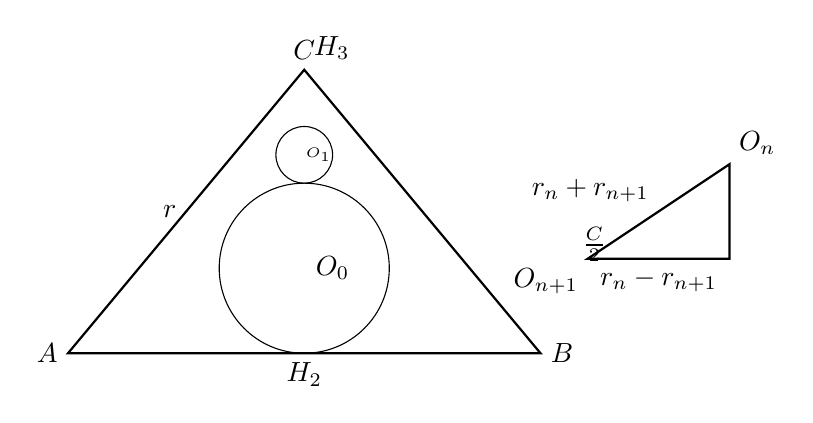
\begin{tikzpicture}[scale=1.2]
    % Triangle ABC
    \coordinate (C) at (0, 3);
    \coordinate (A) at (-2.5, 0);
    \coordinate (B) at (2.5, 0);

    \draw[thick] (A) node[left] {$A$} -- (B) node[right] {$B$} -- (C) node[above] {$C$} -- cycle;
    \draw (C) node[above right] {$H_3$};

    % Incircle C_0
    \draw (0, 0.9) circle (0.9);
    \node at (0.3, 0.9) {$O_0$};

    % Smaller circle C_1 near C
    \draw (0, 2.1) circle (0.3);
    \node at (0.15, 2.1) {\tiny $O_1$};

    % Labels
    \node[left] at (-1.25, 1.5) {$r$};
    \node[below] at (0, 0) {$H_2$};

    % Auxiliary right triangle figure
    \begin{scope}[shift={(3, 1)}]
        \draw[thick] (0,0) -- (1.5,0) node[midway, below] {$r_n - r_{n+1}$} -- (1.5, 1) -- cycle;
        \node[above left] at (0.75, 0.5) {$r_n + r_{n+1}$};
        \node[left] at (0.3, 0.15) {$\frac{C}{2}$};
        \node[above right] at (1.5, 1) {$O_n$};
        \node[below left] at (0, 0) {$O_{n+1}$};
    \end{scope}
\end{tikzpicture}
\end{center}
\end{proof}

\section*{第4問}

\begin{proof}[解]
$\angle AOQ = \theta \quad (0 < \theta \leqq \pi/2)$ とおく. この時, かかる時間 $f(\theta)$ は
\[
f(\theta) = \frac{\breve{AQ}}{2} + \frac{\overline{BQ}}{1} \qquad \dots \text{\textcircled{1}}
\]
である.
\[
\breve{AQ} = \sqrt{3} \theta \qquad \dots \text{\textcircled{2}}
\]
で, $\triangle OBQ$ に余弦定理を用いて,
\[
\overline{BQ}^2 = 1 + 3 - 2\sqrt{3} \cos\left(\frac{\pi}{2} - \theta\right) = 4 - 2\sqrt{3} \sin\theta
\]
\[
\therefore \overline{BQ} = \sqrt{4 - 2\sqrt{3} \sin\theta} \qquad \dots \text{\textcircled{3}}
\]
だから, \textcircled{2}\textcircled{3}を\textcircled{1}に代入して
\[
f(\theta) = \frac{\sqrt{3}}{2} \theta + \sqrt{4 - 2\sqrt{3} \sin\theta}
\]
\[
f'(\theta) = \frac{\sqrt{3}}{2} + \frac{-2\sqrt{3}\cos\theta}{2\sqrt{4 - 2\sqrt{3}\sin\theta}}
\]
とする.
\[
f'(\theta) \geqq 0 \iff \sqrt{4 - 2\sqrt{3} \sin\theta} \geqq 2 \cos\theta
\]
$0 \leqq \theta \leqq \pi/2$ から両辺 $0$ 以上だから2乗して,
\[
4 - 2\sqrt{3} \sin\theta \geqq 4 \cos^2\theta = 4 - 4 \sin^2\theta
\]
\[
\therefore \frac{\sqrt{3}}{2} \leqq \sin\theta \leqq 1 \quad (\because 0 \leqq \sin\theta \leqq 1)
\]
\[
\therefore \frac{\pi}{3} \leqq \theta \leqq \frac{\pi}{2}
\]
となるので, 下表をうる.

\begin{center}
\begin{tabular}{c|ccccc}
$\theta$ & $0$ & $\dots$ & $\pi/3$ & $\dots$ & $\pi/2$ \\ \hline
$f'$ & & $-$ & $0$ & $+$ & \\ \hline
$f$ & & $\searrow$ & & $\nearrow$ & 
\end{tabular}
\end{center}

したがって, もとめる $Q$ の位置は, $\angle QOA = \dfrac{\pi}{3}$ となる場所.

\begin{center}
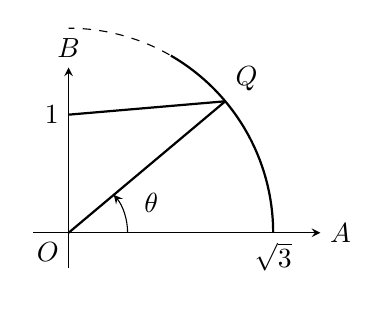
\begin{tikzpicture}[scale=1.5, >=stealth]
    \coordinate (O) at (0,0);
    \coordinate (A) at ({sqrt(3)}, 0);
    \coordinate (B) at (0, 1);
    \coordinate (Q) at ({sqrt(3)*cos(40)}, {sqrt(3)*sin(40)});

    \draw[->] (-0.3,0) -- ({sqrt(3)+0.4},0) node[right] {$A$};
    \draw[->] (0,-0.3) -- (0, 1.4) node[above] {$B$};
    \node[below left] at (O) {$O$};
    \node[below] at (A) {$\sqrt{3}$};
    \node[left] at (B) {$1$};

    % Arc from A to (0, sqrt(3))
    \draw[dashed] ({sqrt(3)}, 0) arc (0:90:{sqrt(3)});
    \draw[thick] (A) arc (0:60:{sqrt(3)});

    \draw[thick] (O) -- (Q) node[above right] {$Q$};
    \draw[thick] (B) -- (Q);

    % Angle theta
    \draw[->] (0.5,0) arc (0:40:0.5);
    \node at (0.7, 0.25) {$\theta$};
\end{tikzpicture}
\end{center}
\end{proof}

\section*{第5問}

\begin{proof}[解]
\[
\int_{-1}^1 f(t) \, dt = 2 \int_0^1 b \, dt = 2b = 1 \implies b = \frac{1}{2}
\]
\[
\int_{-1}^1 x f(x) \, dx = 2 \int_0^1 a x^2 \, dx = \frac{2}{3} a = 0 \implies a = 0
\]
だから, $f(x) = \frac{1}{2}$ であるので,
\[
G(t) = \frac{1}{2} (t+1), \quad A = \int_{-1}^1 \frac{1}{2} x^2 \, dx = \int_0^1 x^2 \, dx = \frac{1}{3}
\]
から
\[
H(t) = \frac{1}{1 + 3t^2}
\]
で, $G(t) > 0, H(t) > 0$ から, $F(t) = \dfrac{G(t)}{H(t)}$ とおくと
\[
F(t) = \frac{1}{2}(t+1)(3t^2+1) = \frac{1}{2}(3t^3 + 3t^2 + t + 1)
\]
\[
2F'(t) = (3t+1)^2 \geqq 0
\]
から, $F(t)$ は単調増加で, $F(0) = \frac{1}{2}$ から, $-1 \leqq t \leqq 0$ では $F(t) \leqq \frac{1}{2} < 1 \quad \therefore G(t) < H(t)$ となる.
\end{proof}

\section*{第6問}

\begin{proof}[解]
\begin{enumerate}
    \item[(1)] 
    \[
    \int_0^1 f(x) \, dx = \frac{1}{4} + \frac{a}{3} + \frac{b}{2} + c \qquad \dots \text{\textcircled{1}}
    \]
    \[
    \sum_{k=1}^n f\left(\frac{k}{n}\right) = \sum_{k=1}^n \left[ \frac{1}{n^3} k^3 + \frac{a}{n^2} k^2 + \frac{b}{n} k + c \right]
    \]
    \[
    = \frac{1}{n^3} \left\{ \frac{n(n+1)}{2} \right\}^2 + \frac{a}{n^2} \frac{1}{6} n(n+1)(2n+1) + \frac{b}{n} \frac{1}{2} n(n+1) + cn
    \]
    \[
    = \frac{(n+1)^2}{4n} + \frac{a}{6} \frac{(n+1)(2n+1)}{n} + \frac{b}{2}(n+1) + cn
    \]
    \[
    = \frac{1}{4}\left(n + 2 + \frac{1}{n}\right) + \frac{a}{6}\left(2n + 3 + \frac{1}{n}\right) + \frac{b}{2}(n+1) + cn
    \]
    \[
    = \left(\frac{1}{4} + \frac{a}{3} + \frac{b}{2} + c\right) n + \left(\frac{1}{2} + \frac{a}{2} + \frac{b}{2}\right) + \left(\frac{1}{4} + \frac{a}{6}\right) \frac{1}{n} \qquad \dots \text{\textcircled{2}}
    \]
    \textcircled{1}\textcircled{2}から
    \[
    n \int_0^1 f(x) \, dx - \sum_{k=1}^n f\left(\frac{k}{n}\right) = -\left(\frac{1}{2} + \frac{a}{2} + \frac{b}{2}\right) - \left(\frac{1}{4} + \frac{a}{6}\right) \frac{1}{n} \xrightarrow{n \to \infty} -\frac{a+b+1}{2}
    \]

    \item[(2)] 
    \[
    f(1+h) - f(1) = \{(1+h)^3 - 1\} + a\{(1+h)^2 - 1\} + b\{(1+h) - 1\}
    \]
    \[
    = (h^3 + 3h^2 + 3h) + a(h^2 + 2h) + bh
    \]
    \[
    f'(x) = 3x^2 + 2ax + b
    \]
    から
    \[
    \frac{f(1+h) - f(1)}{h^2} - \frac{f'(1)}{h} = h + (3+a) + \frac{3+2a+b}{h} - \frac{3+2a+b}{h}
    \]
    \[
    = h + (3+a) \xrightarrow{h \to 0} 3+a
    \]
\end{enumerate}
\end{proof}

\end{document}
